\paragraph{Push- oder Pull-Model} 


Bei den beiden Modellen werden die unterschiedlichen Arten der Übertragung von Daten betrachtet. Bei dem Push-Model ist die Idee, alle Daten über die Update-Methode der Observer zu übermitteln. In unserem Fall muss das UML-Diagramm in Abbildung \ref{observerdiagramm} angepasst werden. Die Methode \texttt{update()} benötigt  zusätzliche Parameter. Das \texttt{ConcreteSubject} übergibt dann die Parameter beim Aufruf der Update-Methode.
Daraus ergeben sich zwei Nachteile. Der Erste, das Subject muss die Observer besser kennen. Die Update-Methode könnte so auf eine bestimmte Aufgabe zugeschnitten werden und somit für andere Anwendungsfälle ungeeignet sein. Der zweite Nachteile ist, das nicht alle Observer diese Informationen benötigen und somit unnötig viele Parameter übermittelt bekommen.
Die Pull Methode verfolgt einen anderen Ansatz. Hier werden keine Daten als Parameter übergeben sondern die Observer greifen direkt nach einer Benachrichtigung auf die Daten der Instanz des \texttt{ConcreteSubject} zu. Der Nachteil dieser Variante ist, das die einzelnen Beobachter das Subjekt kennen müssen und gleichzeitig das Subject öffentliche Methoden für den Zugriff bereitstellen muss.

%\paragraph{Lagerung der Beobachter} Hintegrund ist folgendes Szenario: Es gibt viele Subjekts und einige Beobachter. Die Subjekts müssen jetzt alle die Instanzen der jeweiligen Beobachter speichern. Um sich diesen Speicher zu ersparen, könnte man die Auflistung aller Beobachter in einer externen Datenstruktur bzw. Objekt lagern.

\paragraph{Beobachter beobachtet mehr als ein Subjekt} Wenn ein Observer mehrere Subjects beobachtet, kann es passieren, das er im Falle einer Benachrichtigung nicht feststellen kann, von wem die Update-Methode aufgerufen wurde. Abhilfe schafft die Erweiterung der Update-Methode mit einem zusätzlichen Parameter \texttt{Subject}. Das Subject kann sich bei der Benachrichtigung selbst übermitteln, damit der Observer weiß von wem er benachrichtig wurde. (Siehe Abbildung \ref{observer_update})

\begin{listing}[h!]
   \centering
   \javacode{./resources/observer_erweiterung_update.java}
   \caption{Jobcenter}
    \label{observer_update}
\end{listing} 

\paragraph{Ausführung des Updates} Das Anstoßen der Benachrichtigungen kann entweder vom Client als auch vom konkreten Subject durchgeführt werden. Der Vorteil dies dem konkretem Subject zu überlassen ist die Vermeidung von Fehlern. Fügt man die Notify-Methode nach der Änderung eines Werte in dem Subject ein, wird ein Automatismus geschaffen, sodass die Benachrichtigung nicht vergessen werden kann. Der Nachteil dieser Implementierung ist, das dadurch die Anzahl der Updates höher ausfallen könnte. Die andere Variante überlässt den Client die Verantwortung, nachdem er seine Änderungen übermittelt hat, die Notify-Methode aufzurufen. Hier können zwar die Benachrichtigungen gezielter ausgeführt werden, allerdings könnte die Benachrichtigung auch vergessen werden.

%\paragraph{Aufräumen der Instansen} Es sollte Beachtet werden, das wenn ein Beobachter sich vom konkreten Objekt entfernt, auch die Instanz des konkreten SUbjekt aufräumt. 

%\paragraph{Vor dem Benachrichtigen das Subjekt zuerst updaten} Bei der Implementierung des konkreten Subjekts sollte beachtet werden, vor der Benachrichtigung der Beobachter, zuerst das Subjekt zu aktualisieren. Gerade bei vererbten Methoden besteht Gefahr eines solchen Szenario.

\paragraph{Erweiterung der Benachrichtigung für ein bestimmtes Interesse} In bestimmten Fällen kann es sein, das ein Beobachter nur auf bestimmte Events benachrichtigt werden möchte. In diesem Fall bietet sich an,  die Methode \texttt{attach(Observer)} um einen weiteren Parameter zu erweitern, damit der Beobachter dadurch das Interesse auf ein bestimmtes Event signalisieren kann. (Siehe Abbildung \ref{observer_update_with_observer})

\begin{listing}[h!]
   \centering
   \javacode{./resources/observer_sortToObserverlist.java}
   \caption{Erweiterte }
    \label{observer_update_with_observer}
\end{listing} 

\paragraph{Die externe Verwaltung der Beobachter} Wenn die Beziehung zwischen den konkreten Subject und den Observer zu komplex wird, empfiehlt sich die Verwaltungsaufgaben zwischen Subject und dessen Observer auszulagern. In der Literatur wird von einem ChangeManager gesprochen. Dieser definiert das Mapping zwischen den Subjects und den Observer, regelt spezielle Aktualisierungsstrategien und übernimmt die Benachrichtigung eines konkreten Subjects für dessen Observer. (Siehe Abbildung \ref{observer_changemanager})



\begin{listing}[h!]
   \centering
   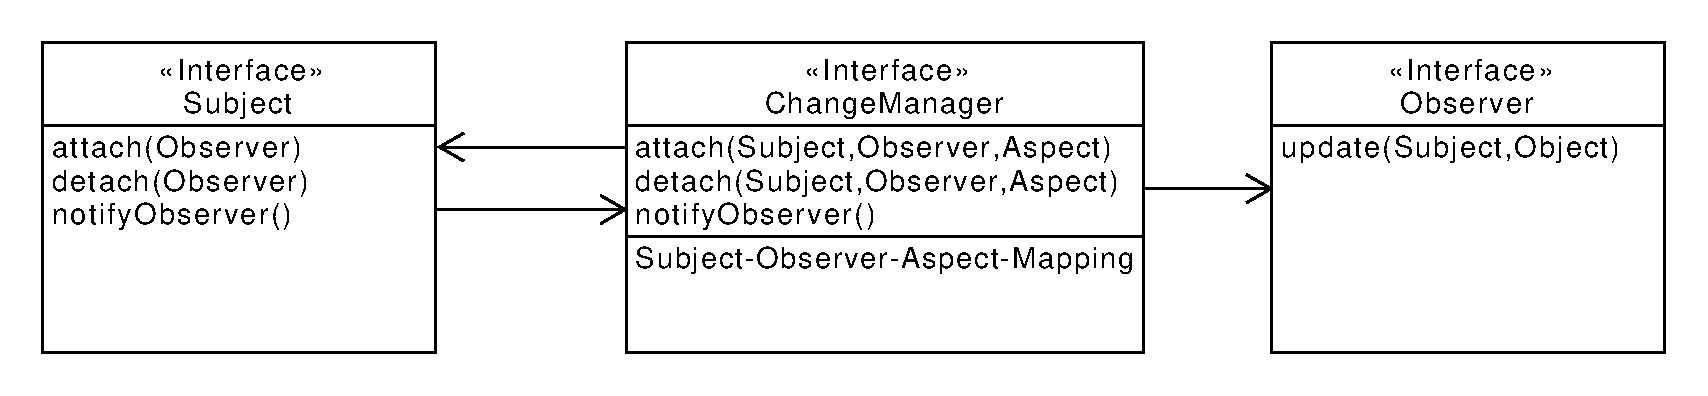
\includegraphics[scale=.4]{paper/observer/changemanager}
   \caption{Changemanager}
    \label{observer_changemanager}
\end{listing} 

%\paragraph{Subjekt als Interface oder Abstrakte Klasse} Das Subjekt kann ein Interface oder als abstrakte klasse implementiert sein. Der Nachteil bei einer abstrakten Klasse ist, dass nicht auf verschiedene konkrete Subjekts eingegangen werden kann. Jedoch erhöht sich der PRogrammieraufwand durch die wiederholte Implementierung des Selben Codes.


